\documentclass[border=3pt]{standalone}
\usepackage[T1]{fontenc}
\usepackage[utf8]{inputenc}
\usepackage{lmodern}
\usepackage{amsmath,amssymb}
\usepackage{xcolor}
\usepackage{tikz}
\usepackage{fontawesome5}
\usepackage{ragged2e}
\usetikzlibrary{shapes,shapes.geometric,shapes.misc,arrows.meta,positioning,
                calc,fit,backgrounds,decorations.pathreplacing,
                decorations.markings,patterns,chains}
\usetikzlibrary{decorations.pathreplacing,decorations.markings}
\definecolor{primary}{HTML}{1A5276}
\definecolor{secondary}{HTML}{2E86C1}
\definecolor{accent}{HTML}{E74C3C}
\definecolor{lightbg}{HTML}{EBF5FB}
\definecolor{defbg}{HTML}{FDF2E9}
\definecolor{greenhl}{HTML}{27AE60}
\definecolor{purplehl}{HTML}{8E44AD}
\definecolor{goldhl}{HTML}{B7950B}
\definecolor{tealhl}{HTML}{117A65}
\definecolor{codebg}{HTML}{F4F6F7}
\definecolor{neutral}{HTML}{707B7C}
\definecolor{dom1}{HTML}{1F618D}
\definecolor{dom2}{HTML}{117864}
\definecolor{dom3}{HTML}{6C3483}
\definecolor{dom4}{HTML}{922B21}
\definecolor{dom5}{HTML}{B7950B}
% --- carried over from ccna.sty so figures match the book exactly
\tikzset{
  dev/.style={rounded corners=3pt, draw=#1, fill=#1!8, text=#1!45!black,
              line width=0.9pt, minimum width=1.45cm, minimum height=1.05cm,
              align=center, font=\scriptsize\bfseries, inner sep=2pt},
  wirestyle/.style={line width=0.9pt, neutral!75},
  xconn/.style={line width=0.9pt, neutral!75, dash pattern=on 2.5pt off 2pt},
}

\newcommand{\Rtr}[3]{\node[dev=dom3] (#1) at #2 {\faIcon{route}\\#3};}
\newcommand{\Sw}[3]{\node[dev=dom2] (#1) at #2 {\faIcon{sitemap}\\#3};}
\newcommand{\Msw}[3]{\node[dev=dom3] (#1) at #2 {\faIcon{layer-group}\\#3};}
\newcommand{\Host}[3]{\node[dev=neutral] (#1) at #2 {\faIcon{desktop}\\#3};}
\newcommand{\Lap}[3]{\node[dev=neutral] (#1) at #2 {\faIcon{laptop}\\#3};}
\newcommand{\Srv}[3]{\node[dev=dom1] (#1) at #2 {\faIcon{server}\\#3};}
\newcommand{\Ap}[3]{\node[dev=dom5] (#1) at #2 {\faIcon{wifi}\\#3};}
\newcommand{\Wlc}[3]{\node[dev=dom5] (#1) at #2 {\faIcon{broadcast-tower}\\#3};}
\newcommand{\Fw}[3]{\node[dev=dom4] (#1) at #2 {\faIcon{shield-alt}\\#3};}
\newcommand{\Cld}[3]{\node[dev=neutral] (#1) at #2 {\faIcon{cloud}\\#3};}
\newcommand{\Phone}[3]{\node[dev=dom5] (#1) at #2 {\faIcon{phone-alt}\\#3};}
\newcommand{\Prn}[3]{\node[dev=neutral] (#1) at #2 {\faIcon{print}\\#3};}

% A link. The optional argument takes tikz options (e.g. xconn for a
% trunk drawn dashed); the fourth argument labels the link.
\newcommand{\wire}[4][wirestyle]{%
  \draw[#1] (#2) -- node[font=\tiny, text=neutral!85!black, fill=white,
                          inner sep=1.2pt, midway] {#4} (#3);}
\newcommand{\plainwire}[3][wirestyle]{\draw[#1] (#2) -- (#3);}


\newenvironment{topology}[1][]
  {\begin{center}\begin{tikzpicture}[font=\scriptsize,#1]}
  {\end{tikzpicture}\end{center}}


\newcommand{\cmd}[1]{\texttt{\small #1}}
\newcommand{\term}[1]{\textbf{\textcolor{primary}{#1}}}
\newcommand{\chref}[1]{Chapter~\ref{ch:#1}}
\newcommand{\ccnafitw}[1]{#1}
\providecommand{\thefigure}{}
% --- progressive builds
\newcount\buildlevel \buildlevel=99
% \stepvis{n}{..} appears from level n onward; \steponly{n}{..} at
% level n alone, which is how a caption is swapped rather than
% accumulated as the build advances. \stepdim{n}{..} is the
% complement of \stepvis: it shows only BEFORE level n, so a
% pair of them draws an element faint and then solid. That keeps
% the canvas full from step 1, which matters for a figure whose
% shape is itself the lesson -- a five-rung ladder revealed one
% rung at a time leaves a void where the method should be.
\newcommand{\stepvis}[2]{\ifnum#1>\buildlevel\relax\else#2\fi}
\newcommand{\steponly}[2]{\ifnum#1=\buildlevel #2\fi}
\newcommand{\stepdim}[2]{\ifnum#1>\buildlevel #2\fi}
% Slide text does not hyphenate. A projected caption broken as
% ``uni-cast'' costs the reader a beat that print can afford and a
% lecture cannot, and the ragged edge it avoids is invisible at
% four metres anyway.
\hyphenpenalty=10000 \exhyphenpenalty=10000
\begin{document}
\buildlevel=6
% Slide build of Figure 33.1 -- the seven-step cycle, one step at a time.
%
% This is the figure the whole of Part VI hangs on, and the one a student is
% most likely to photograph and never look at again. Built, it stops being a
% poster and becomes a rehearsal: each step arrives with the sentence that
% says what it costs to skip it.
%
% Ghosts, as with the reachability ladder: the shape is the lesson. A student
% who cannot see that there are seven steps has no reason to believe the order
% matters, and the empty slots make "which ones do people skip?" a question the
% room can answer before being told (it is 1, 2 and 5).
%
% The return arc waits for step 6, because until there is a test there is
% nothing to fail -- and that arc is the point of the whole diagram.
%
% The solid nodes carry names and the arrows between them are drawn by name,
% exactly as the book draws them; only the faint placeholders use coordinates,
% since a \draw naming a node that a lower build level has not drawn is an
% undefined-node error rather than a missing arrow.
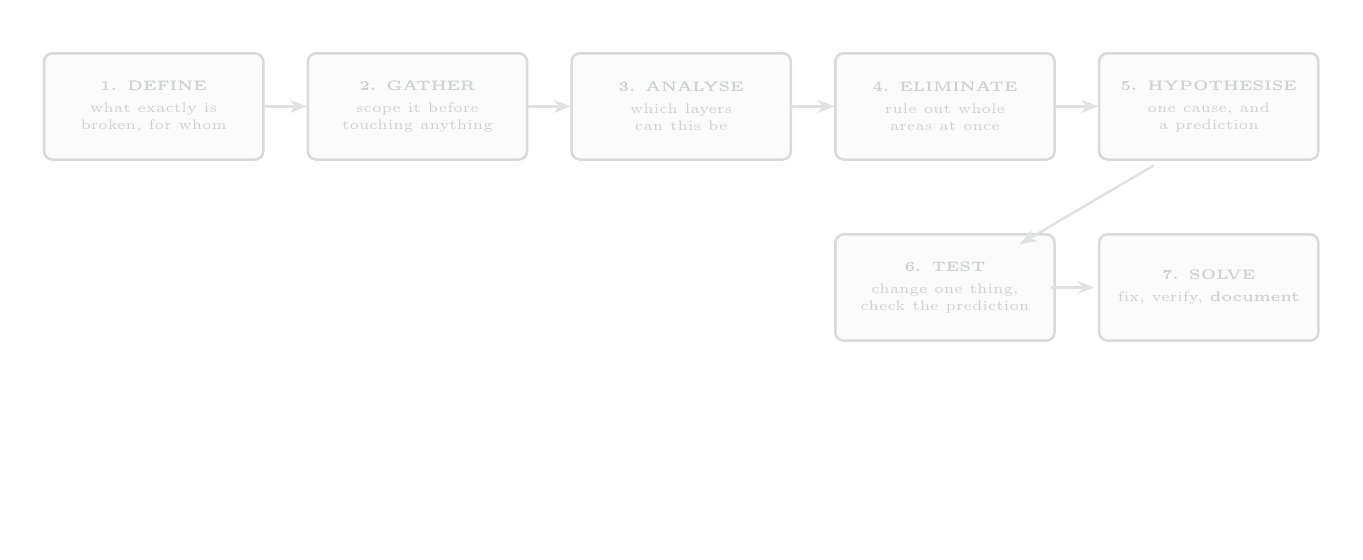
\begin{tikzpicture}[font=\scriptsize]
  \path (-1.6,-5.4) rectangle (15.0,1.0);

  \tikzset{
    st/.style={rounded corners=3pt, draw=#1, fill=#1!8, text=#1!45!black,
               line width=0.9pt, text width=2.55cm, align=center,
               minimum height=1.35cm, font=\tiny\bfseries},
    ghost/.style={rounded corners=3pt, draw=neutral!28, fill=neutral!3,
                  text=neutral!35, line width=0.9pt, text width=2.55cm,
                  align=center, minimum height=1.35cm, font=\tiny\bfseries},
    a/.style={-{Stealth[length=2.2mm]}, line width=0.9pt, neutral!70},
    dim/.style={-{Stealth[length=2.2mm]}, line width=0.9pt, neutral!22},
    stepcap/.style={font=\bfseries, anchor=north west, text width=16.2cm,
                    align=left}}

  % --- the seven stations, ghosted until reached ------------------------
  \stepdim{1}{\node[ghost] at (0,0) {1. DEFINE\\[2pt]\mdseries what exactly is
      broken, for whom};}
  \stepvis{1}{\node[st=dom1] (s1) at (0,0) {1. DEFINE\\[2pt]\mdseries what
      exactly is broken, for whom};}

  \stepdim{2}{\node[ghost] at (3.35,0) {2. GATHER\\[2pt]\mdseries scope it
      before touching anything};}
  \stepvis{2}{\node[st=dom1] (s2) at (3.35,0) {2. GATHER\\[2pt]\mdseries scope
      it before touching anything};}

  \stepdim{3}{\node[ghost] at (6.7,0) {3. ANALYSE\\[2pt]\mdseries which layers
      can this be};}
  \stepvis{3}{\node[st=dom1] (s3) at (6.7,0) {3. ANALYSE\\[2pt]\mdseries which
      layers can this be};}

  \stepdim{4}{\node[ghost] at (10.05,0) {4. ELIMINATE\\[2pt]\mdseries rule out
      whole areas at once};}
  \stepvis{4}{\node[st=dom1] (s4) at (10.05,0) {4. ELIMINATE\\[2pt]\mdseries
      rule out whole areas at once};}

  \stepdim{5}{\node[ghost] at (13.4,0) {5. HYPOTHESISE\\[2pt]\mdseries one
      cause, and a prediction};}
  \stepvis{5}{\node[st=dom4] (s5) at (13.4,0) {5. HYPOTHESISE\\[2pt]\mdseries
      one cause, and a prediction};}

  \stepdim{6}{\node[ghost] at (10.05,-2.3) {6. TEST\\[2pt]\mdseries change one
      thing, check the prediction};}
  \stepvis{6}{\node[st=dom4] (s6) at (10.05,-2.3) {6. TEST\\[2pt]\mdseries
      change one thing, check the prediction};}

  \stepdim{7}{\node[ghost] at (13.4,-2.3) {7. SOLVE\\[2pt]\mdseries fix,
      verify, \textbf{document}};}
  \stepvis{7}{\node[st=dom2] (s7) at (13.4,-2.3) {7. SOLVE\\[2pt]\mdseries fix,
      verify, \textbf{document}};}

  % --- the path ---------------------------------------------------------
  % Each placeholder is retired by the level that draws the real arrow over
  % it. Left in, the hand-placed coordinates do not quite coincide with the
  % node-to-node path, and the 5-to-6 arrow rendered as a faint double.
  \foreach \n/\x in {2/1.4, 3/4.75, 4/8.1, 5/11.45}
    {\stepdim{\n}{\draw[dim] (\x,0) -- ++(0.55,0);}}
  \stepdim{6}{\draw[dim] (12.7,-0.75) -- (11.0,-1.75);}
  \stepdim{7}{\draw[dim] (11.4,-2.3) -- (11.95,-2.3);}

  \stepvis{2}{\draw[a] (s1) -- (s2);}
  \stepvis{3}{\draw[a] (s2) -- (s3);}
  \stepvis{4}{\draw[a] (s3) -- (s4);}
  \stepvis{5}{\draw[a] (s4) -- (s5);}
  \stepvis{6}{\draw[a] (s5) -- (s6);}
  \stepvis{7}{\draw[a] (s6) -- (s7);}

  % --- the loop, which is the whole point ------------------------------
  % The label rides on the arc, on a white ground -- the same fix the book got.
  % Beside it, the label either lands in the gap the arc encloses (the
  % ELIMINATE box) or drifts close enough to the grey 5-to-6 arrow to read as
  % its label instead.
  \stepvis{6}{%
    \draw[a, dom4!70] (s6) to[bend left=30]
        node[font=\tiny, text=dom4!45!black, align=center, midway,
             fill=white, inner sep=1.5pt] {prediction\\failed} (s5);}

  % Caption n describes station n. Written one behind -- as though step 1
  % were an introduction -- every caption named the box to the left of the
  % one that had just lit up.
  \steponly{1}{\node[stepcap, text=dom1!45!black] at (-1.5,-3.5)
      {``The network is down'' is not a fault. Who, what, since when, and what
       still works? Seven steps --- and the three that get skipped under
       pressure are 1, 2 and 5.};}
  \steponly{2}{\node[stepcap, text=dom1!45!black] at (-1.5,-3.5)
      {Scope it \emph{before} touching anything. Once you have changed
       something you can no longer tell what the fault was.};}
  \steponly{3}{\node[stepcap, text=dom1!45!black] at (-1.5,-3.5)
      {Now decide which layers this can possibly be. Most of the stack is
       usually innocent, and saying so out loud is what stops the guessing.};}
  \steponly{4}{\node[stepcap, text=dom1!45!black] at (-1.5,-3.5)
      {Rule out whole areas at once. One ping to the gateway clears layers 1
       to 3 on this segment --- that is four steps of a bottom-up search in a
       single command.};}
  \steponly{5}{\node[stepcap, text=dom4!45!black] at (-1.5,-3.5)
      {\emph{One} cause, and a prediction --- ``if I am right, this command
       will show that''. A guess with no prediction cannot be wrong, which is
       exactly what makes it useless.};}
  \steponly{6}{\node[stepcap, text=dom4!45!black] at (-1.5,-3.5)
      {Change one thing, and check the prediction. If it failed the hypothesis
       is discarded --- not patched --- and you go straight back to 5. That arc
       is the method; everything above it is preparation.};}
  \steponly{7}{\node[stepcap, text=dom2!45!black] at (-1.5,-3.5)
      {And only then fix it. \textbf{Document} is part of step 7, not an
       optional extra: the next person to meet this fault is usually you, six
       months later.};}
\end{tikzpicture}

\end{document}
